\subsubsection{\stid{3.11} ALExa}


\paragraph{Overview}

The ALExa project ({\sl Accelerated Libraries for
Exascale})
focuses on preparing the DTK and Tasmanian libraries for
exascale platforms and integrating these libraries into ECP
applications.  These libraries deliver capabilities
identified as needs of ECP applications: (1) the ability to
transfer computed solutions between grids with differing
layouts on parallel accelerated architectures,
enabling simulation projects such as ExaAM and ExaSMR to
seamlessly combine results from different computational
grids to perform their required simulations (DTK); and
%
(2) the ability to construct fast and memory efficient
surrogates to large scale engineering models with
multiple inputs and large number of outputs, enabling
uncertainty quantification (both forward and inverse)
as well as optimization and efficient multi-physics
simulations in projects such as ExaStar (Tasmanian).

These capabilities
are being developed through ongoing interactions with our
ECP application project collaborators to ensure they will
satisfy requirements of these customers.  The libraries in
turn take advantage of other ECP/SW capabilities currently in
development, including Trilinos, Kokkos and SLATE.  The
final outcome of the ECP project will be a set of
libraries deployed to facilities
and also made broadly available as part of the xSDK4ECP
project.

{\bf DTK} (Data Transfer Kit)
{\it Purpose:}
Transfers computed solutions between grids with differing
layouts on parallel accelerated architectures.
{\it Significance:} Coupled applications frequently have
different grids with different parallel distributions; DTK
is able to transfer solution values between these grids
efficiently and accurately.
{\it Mesh-free interpolation capabilities:}
multivariate data interpolation between point clouds;
compactly supported radial basis functions;
nearest-neighbor and moving least square implementations;
common applications include conjugate heat transfer,
fluid structure interaction, and mesh deformation.
{\it Performance portable search capabilities:}
threaded and GPU implementations of spatial tree
construction;
threaded and GPU implementations of various spatial tree
queries;
MPI front-end for coordinating distributed spatial searches
between sets of geometric objects with different
decompositions;
communication plan generation based on spatial search
results.
{\it URL:}
https://github.com/ORNL-CEES/DataTransferKit

{\bf Tasmanian} (Toolkit for Adaptive Stochastic Modeling
and Non-Intrusive Approximation)
{\it Purpose:} Constructs efficient surrogate models for high
dimensional problems and performs parameter calibration
and optimization geared towards applications in
uncertainty quantification (UQ).
{\it Significance:}
UQ pertains to the statistical properties of the output from
a complex model with respect to variability in multiple
model inputs; large number of simulations are required to compute
reliable statistics which is prohibitive when dealing with
computationally expensive engineering models. A surrogate model
is constructed from a moderate set of simulations using carefully
chosen input values; analysis can then be performed on the efficient surrogate.
{\it Sparse grids capabilities:}
surrogate modeling and design of experiments (adaptive
multi-dimensional interpolation);
reduced (lossy) representation of tabulated scientific data;
high dimensional numerical quadrature;
data mining and manifold learning.
{\it DiffeRential Evolution Adaptive Metropolis (DREAM)
capabilities:}
Bayesian inference;
parameter estimation/calibration;
model validation.
global optimization and optimization under uncertainty.
{\it URL:}
http://tasmanian.ornl.gov

\paragraph{Key Challenges}

\indent

{\bf DTK:}
The general case of transferring data between grids of
unrelated applications requires an all-to-all
communication.
This is increasingly challenging as communication
to computation ratios are decreasing on successive HPC
systems.
Furthermore, the grid cell search procedures to locate
interpolation points require tree search methods
difficult to optimize on modern accelerated
architectures due to vector lane or thread divergence.
Also, maintaining high accuracy for the transfer requires
careful attention to the mathematical properties of the
interpolation methods and is highly application-specific.
Unlike other, ``black box'' libraries,
grid transfer methods may require close collaboration
with application partners to understand customer
requirements
(accuracy and conservation law requirements,
distribution of grids, location and layout of grid data in
memory hierarchy, etc.)

{\bf Tasmanian:}
Complex models usually have significant variability in execution time
for different model inputs, which leads to massive down-time when
employing the standard fork-join adaptive sparse grid algorithms.
After the surrogate has been constructed, collecting the samples
for statistical analysis (or multi-physics simulations)
requires a massive number of basis evaluations
and many sparse and dense linear operations.

\paragraph{Solution Strategy}

\nobreak


\indent

{\bf DTK:}
State of the art mathematically rigorous methods are used in
DTK to preserve accuracy of interpolated solutions.
Algorithms are implemented in a C++ code base with extensive
unit testing on multiple platforms.
Trilinos packages are used to support interpolation methods.
Kokkos is used to achieve performance portability
across accelerated platforms.

{\bf Tasmanian:}
Implement asynchronous DAG-based sparse grids construction methods
that preserve the convergence properties of the fork-join algorithms
but are insensitive to fluctuations in model simulation time.
Port the basis evaluations and linear algebra to the
GPU accelerators, and leverage the SLATE/MAGMA capabilities
to ensure performance portability across relevant platforms.


%----------------------------------------

\paragraph{Recent Progress}

\indent

{\bf DTK:}
Ongoing work with a growing list of ECP application partners
is continuing.
Extensive work has been done to define the Fortran, C and
C++ DTK interfaces to support partner projects.
A set of benchmark problems has been developed
to guide DTK method and code development.
Recent progress has been made to optimize the search methods
for modern-generation GPUs.

\begin{figure}[htb]
        \centering
        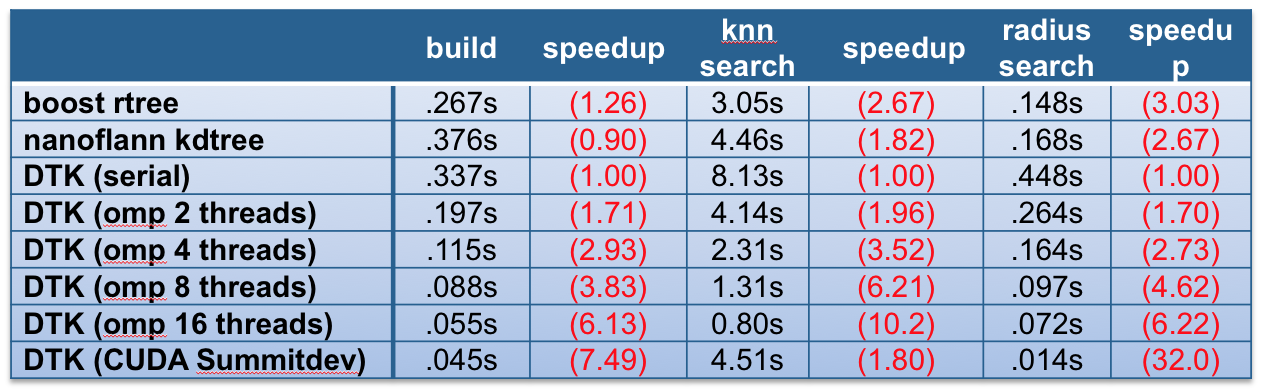
\includegraphics[width=4in]{projects/2.3.3-MathLibs/2.3.3.11-ALExa/dtk-gpu}
        \caption{\label{fig:dtk-gpu}DTK tree search, OpenMP and Summitdev GPU speedups}
\end{figure}

{\bf Tasmanian:}
The infrastructure of Tasmanian has been upgraded to support
the broader ECP focus of the work.
GPU acceleration of sparse grid surrogates has been
implemented.
Tasmanian recently enabled the ExaStar project
to reduce the size of a large-memory table of neutrino
opacities by 100X while still preserving accuracy.

\begin{figure}[htb]
        \centering
        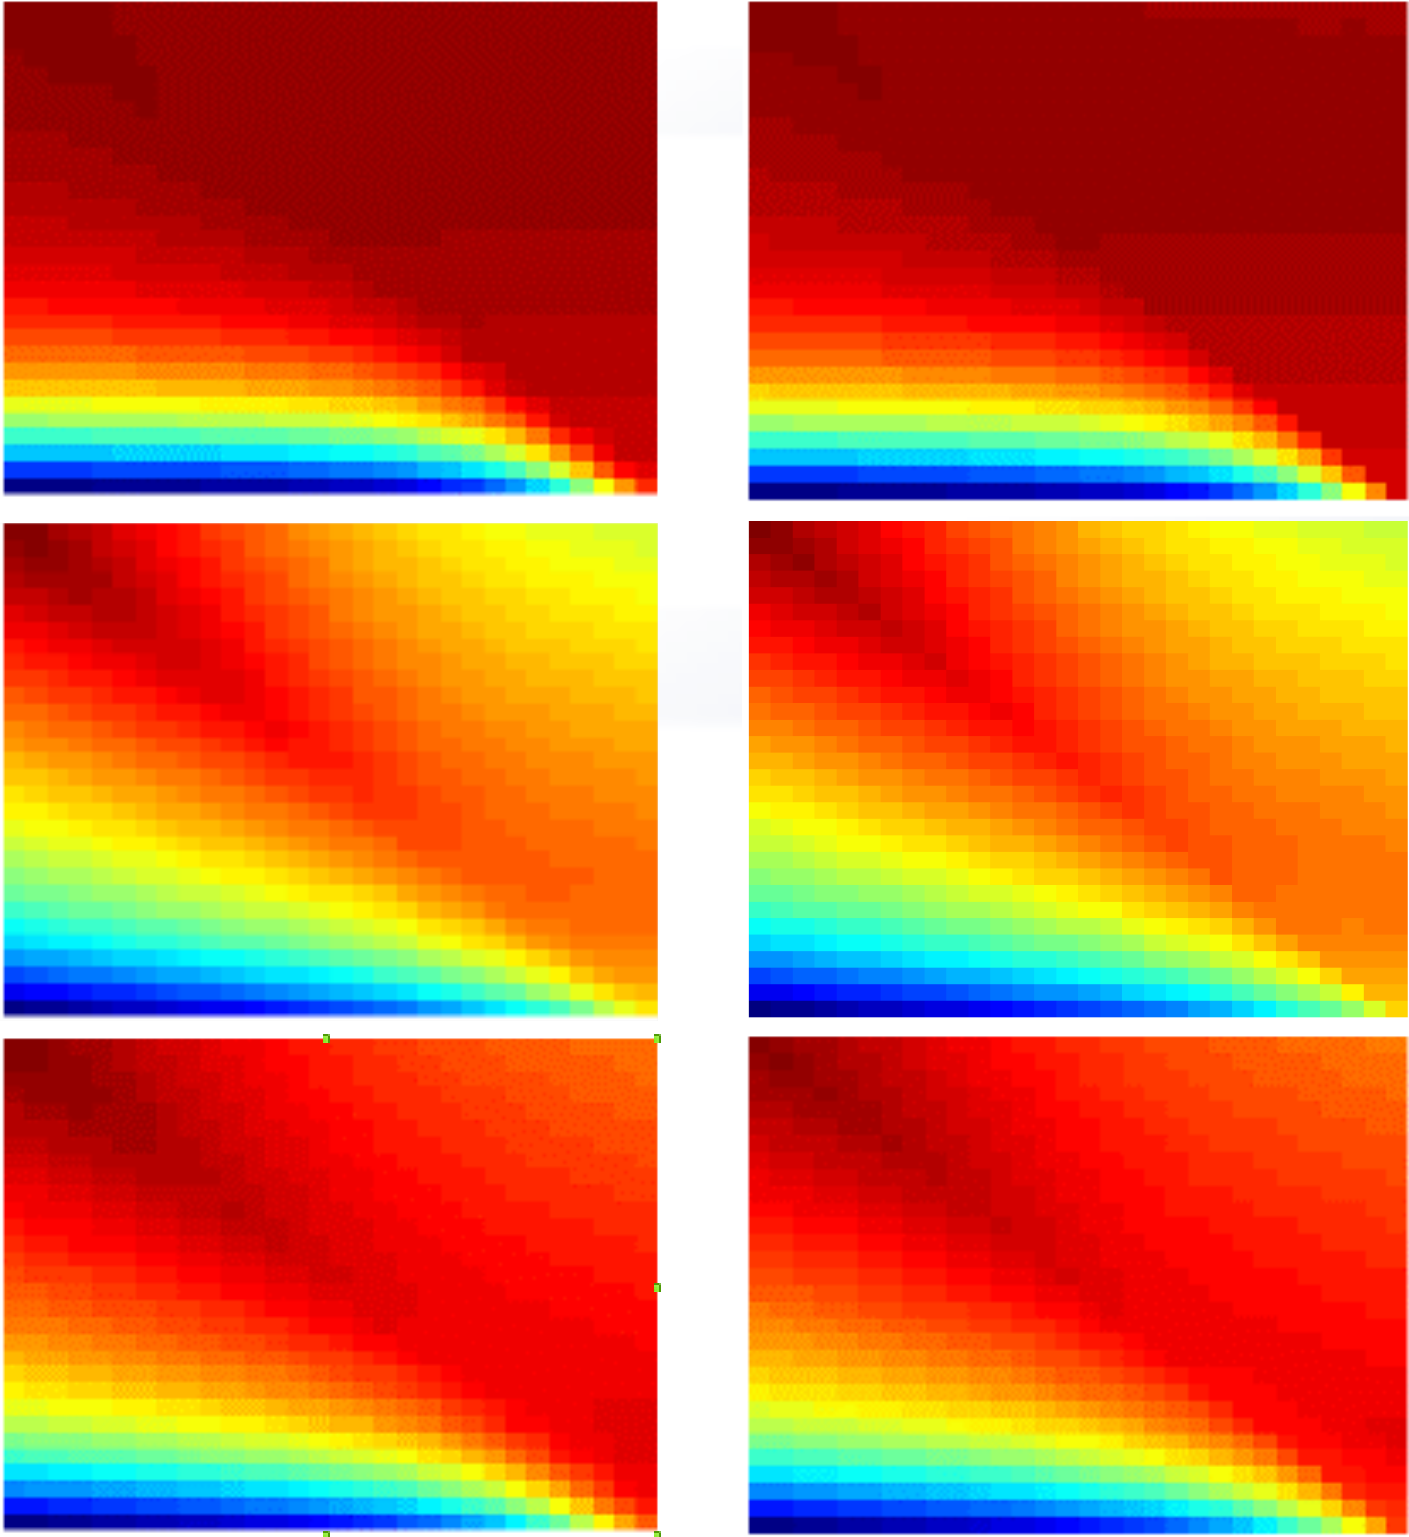
\includegraphics[width=1.5in]{projects/2.3.3-MathLibs/2.3.3.11-ALExa/tasmanian-gpu}
        \caption{\label{fig:tasmanian-gpu}Tasmanian approximation (right) of neutrino capacities (left).}
\end{figure}

%----------------------------------------

\paragraph{Next Steps}

\indent

{\bf DTK:}
A major focus for the near future is to optimize performance
for the targeted architectures using the developed benchmark
cases.
This will be followed by work on a showcase problem to
demonstrate performance.

{\bf Tasmanian:}
Work will continue with the development of the asynchronous
construction methods that exploit the native sparse grids DAG hierarchy.

%----------------------------------------
